\documentclass[solutions]{esg8022pset} 
\usepackage{amsmath}
\usepackage{amssymb}
\usepackage{enumerate}
\usepackage{graphicx}
\usepackage{hyperref}
\usepackage{mathtools}
\usepackage[per-mode=symbol,exponent-product=\cdot]{siunitx} %If this line is giving you trouble, try replacing per-mode with per
\providecommand{\uvec}[1]{{\hat{\bf{#1}}}}
\usepackage{pgf,tikz}
\usetikzlibrary{arrows}
\usepackage{wasysym}
\usepackage{subfig}
\usepackage{wrapfig}
\makeatletter
\newcommand{\interitemtext}[1]{%
  \begin{list}{}
   {\itemindent=0mm\labelsep=0mm
   \labelwidth=0mm\leftmargin=0mm
   \addtolength{\leftmargin}{-\@totalleftmargin}}
    \item #1
  \end{list}
}
\makeatother
\renewcommand{\d}{\,d}
\providecommand{\norm}[1]{\lVert#1\rVert}

\AtBeginDocument{%
  % Appologies to any future editor on the inconsistencies in TeX code and the unnecessary braces.  I'm aggregating previously typeset problems, and didn't think it worth my time to improve the quality of TeX code in ways that won't make any difference to the typeset material. -Jason Gross (jgross@mit.edu)
}%
\classname{Physics 8.022} \semester{Spring 2011} 
\problemsetnumber{7}
\date{\today }
\duedate{Monday, March 28 at 10 \textsc {pm}}
\readingassignment{}
\problemsettitle{Magnetic Force, Special Relativity, Review}
\begin{document}
  \noindent \textbf{Review past concepts \& problems!!!}

  \noindent \textbf{Reading on complex numbers:} \url{http://web.mit.edu/sahughes/www/8.022/complex.pdf}
\section{Problem \thesection: }
\subsection{Problem}
  Particle $A$ with charge $q$ and mass $m_A$ and particle $B$ with charge $2q$ and mass $m_B$, are accelerated from rest by a potential difference $\Delta V$, and subsequently deflected by a uniform magnetic field into semicircular paths. The radii of the trajectories by particle $A$ and $B$ are $R$ and $2R$, respectively. The direction of the magnetic field is perpendicular to the velocity of the particle. What is their mass ratio?
\subsection{Solution}
  (In SI Units)

  The kinetic energy gained by the charges is equal to
  $$\frac12 mv^2 = q\Delta V$$
  which yields
  $$v = \sqrt{\frac{2q \Delta V}{m}}$$
  The charges move in semicircles, since the magnetic force points radially inward and provides the source of the centripetal force:
  $$\frac{mv^2}{r} = qvB$$
  The radius of the circle can be readily obtained as:
  $$r = \frac{mv}{qB} = \frac{m}{qB}\sqrt{\frac{2q\Delta V}{m}} = \frac{1}{B}\sqrt{\frac{2m\Delta V}{q}}$$
  which shows that $r$ is proportional to $\sqrt{m/q}$. The mass ratio can then be obtained from
  $$\frac{r_A}{r_B} = \frac{\sqrt{m_A / q_A}}{\sqrt{m_B / q_B}} \implies \frac{R}{2R} = \frac{\sqrt{m_A / q}}{\sqrt{m_B / 2q}}$$
  which gives
  $$\frac{m_A}{m_B} = \frac18$$
\section{Problem \thesection: }
\subsection{Problem}
  Let us treat the motion of an electron in a hydrogen atom classically. Suppose that an electron follows a circular orbit of radius $r$ around a proton. What is the angular frequency of the orbit $\omega$? Suppose now that a \emph{small} magnetic field perpendicular to the plane of the orbit is switched on. Assuming that the radius of the orbit does not change, calculate the shift in orbital frequency in terms of the magnitude of $B$. This is known as the ``Zeeman effect''.
\subsection{Solution}
  \begin{center}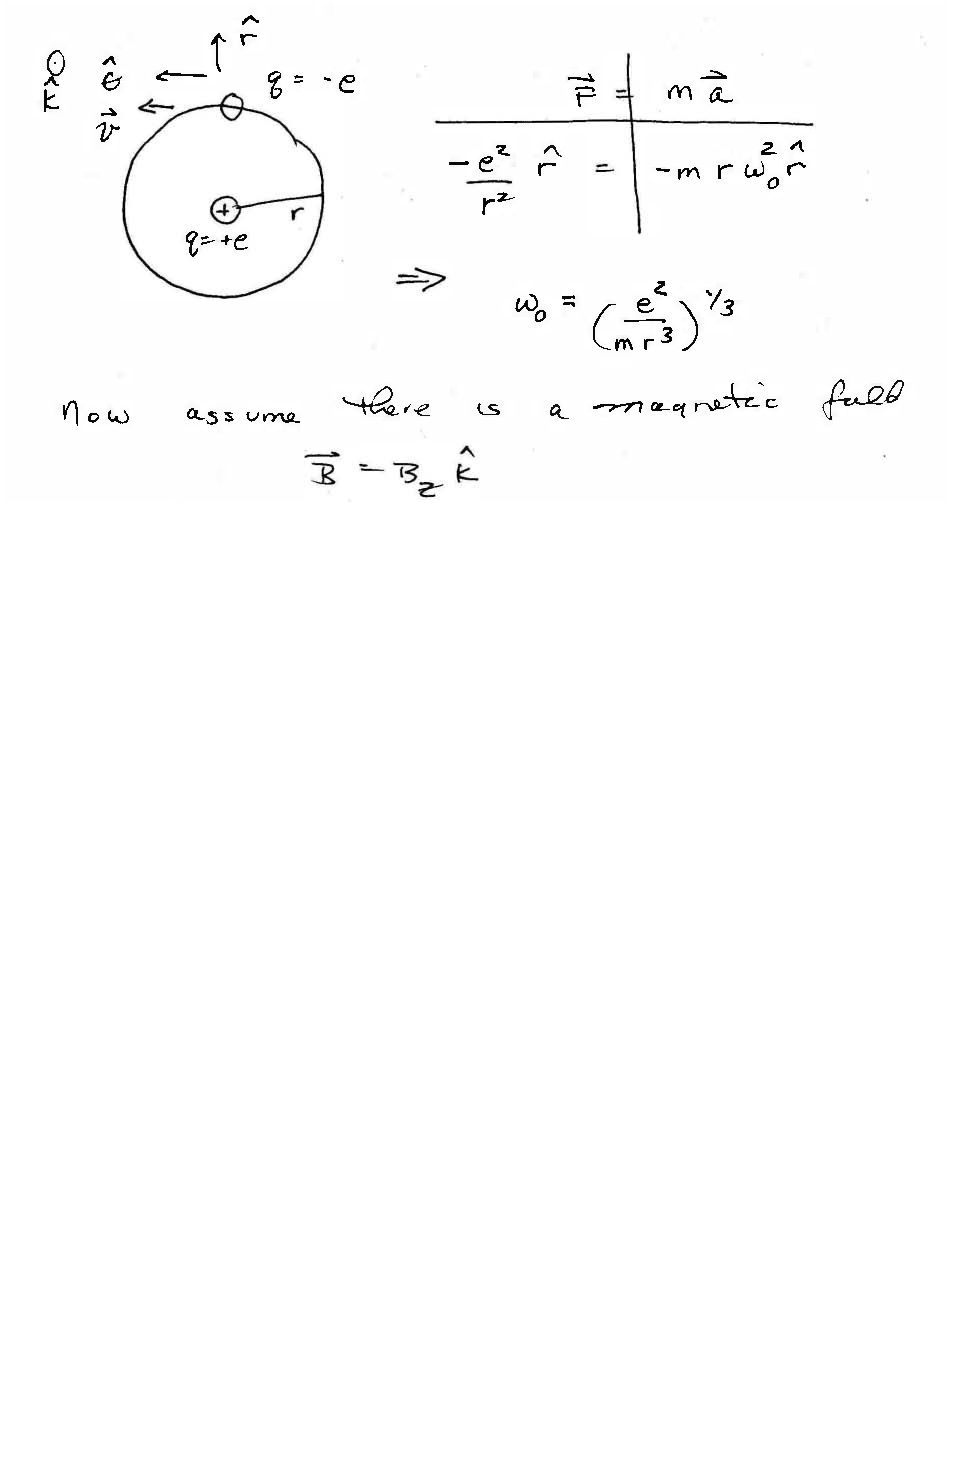
\includegraphics[width=\textwidth]{ps07_sol_02_1.pdf}\end{center}
  \begin{center}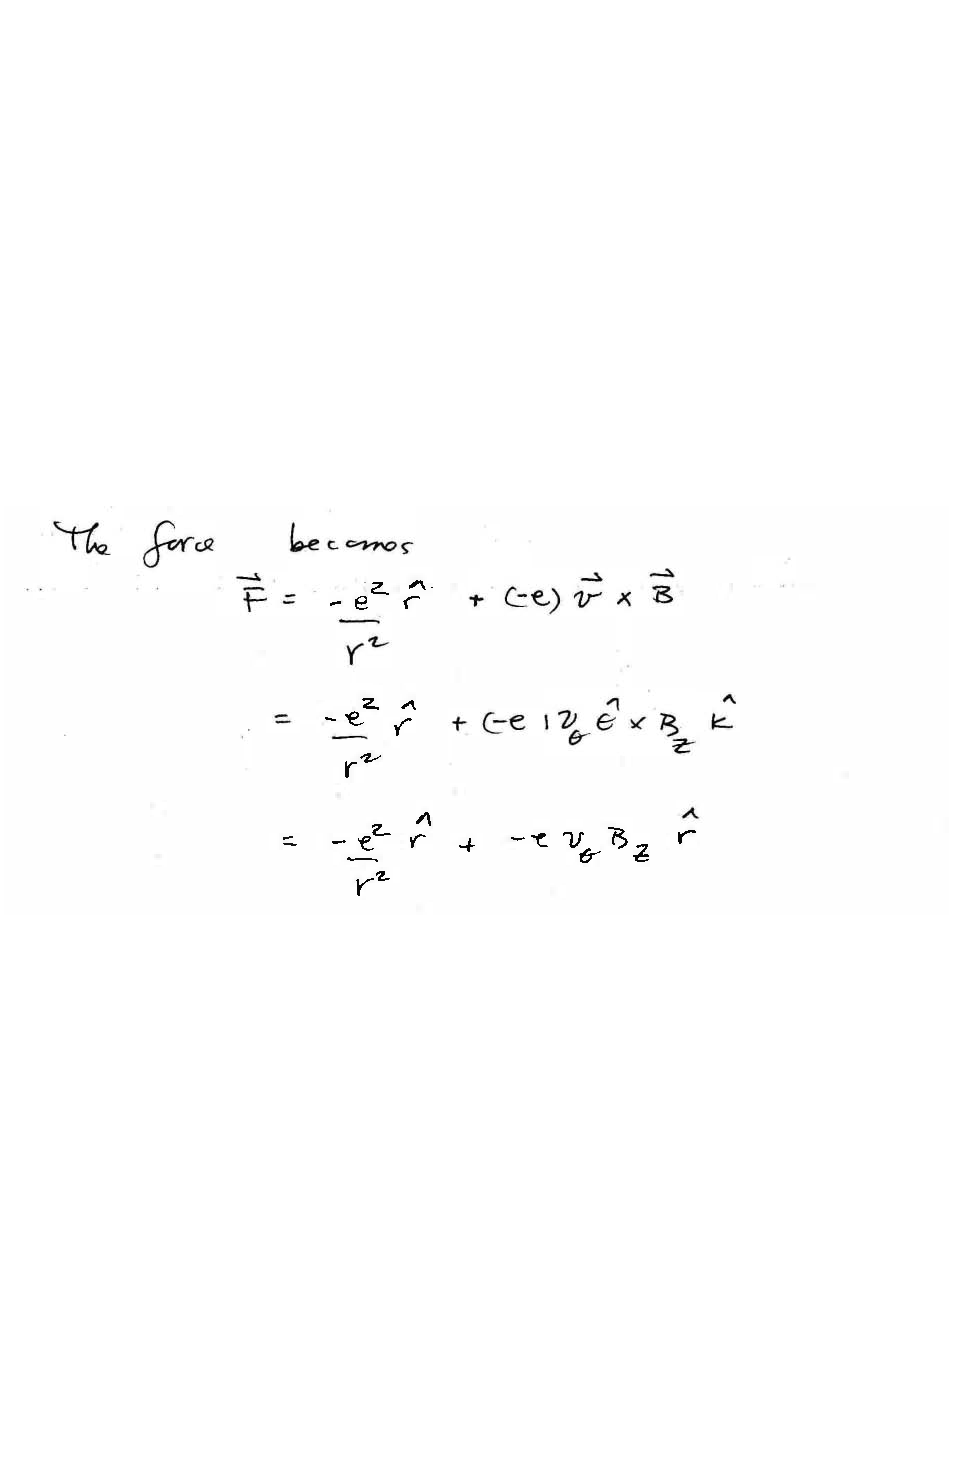
\includegraphics[width=\textwidth]{ps07_sol_02_2.pdf}\end{center}
  \begin{center}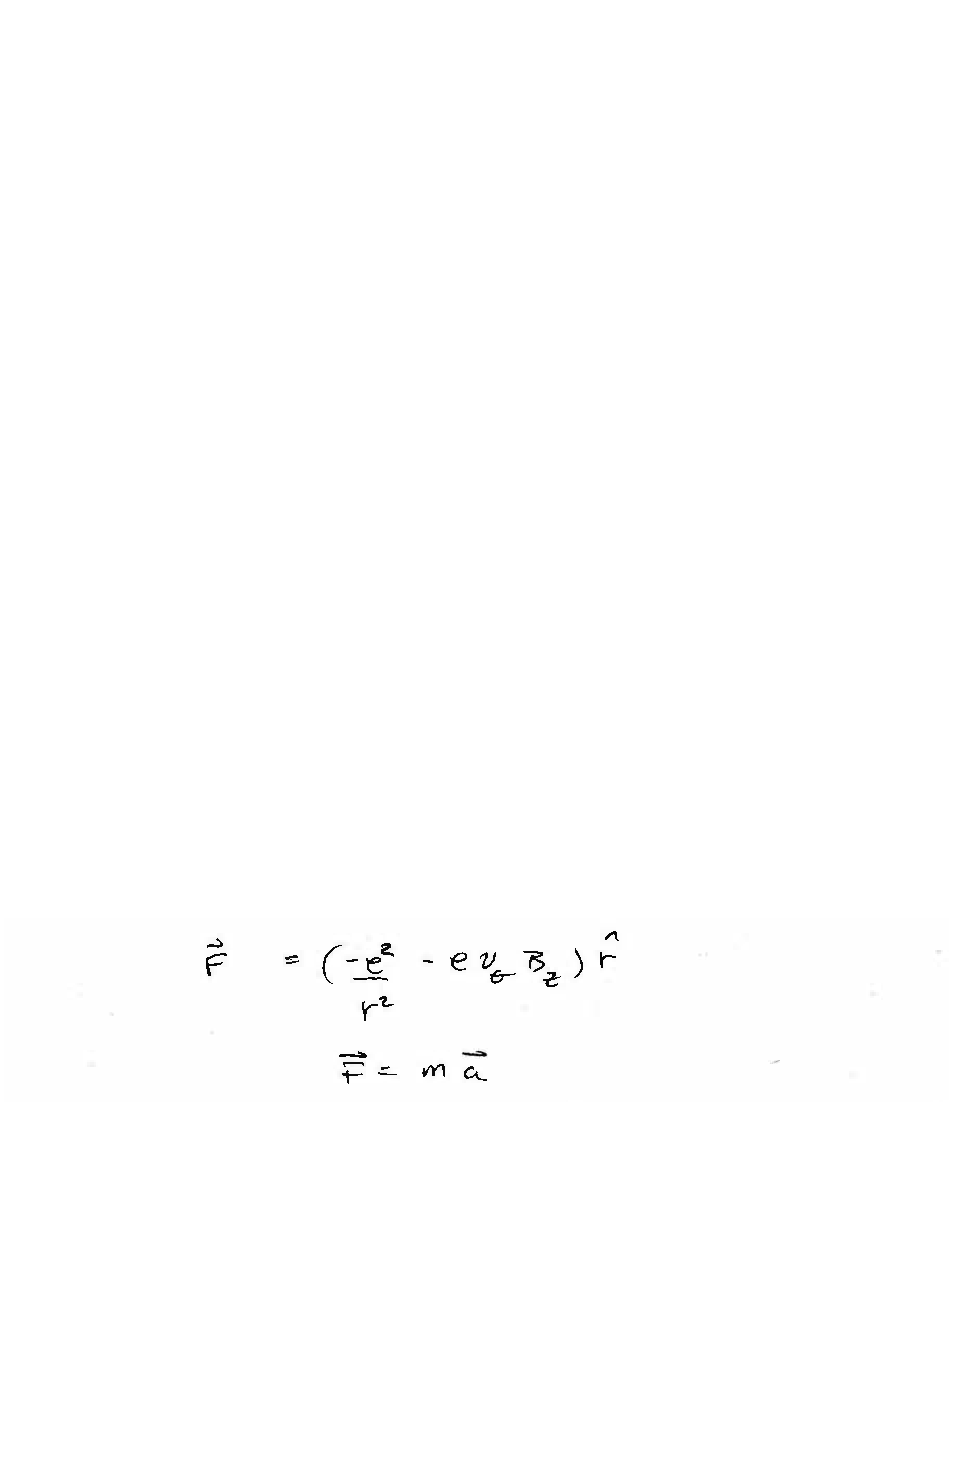
\includegraphics[width=\textwidth]{ps07_sol_02_3.pdf}\end{center}
  \begin{center}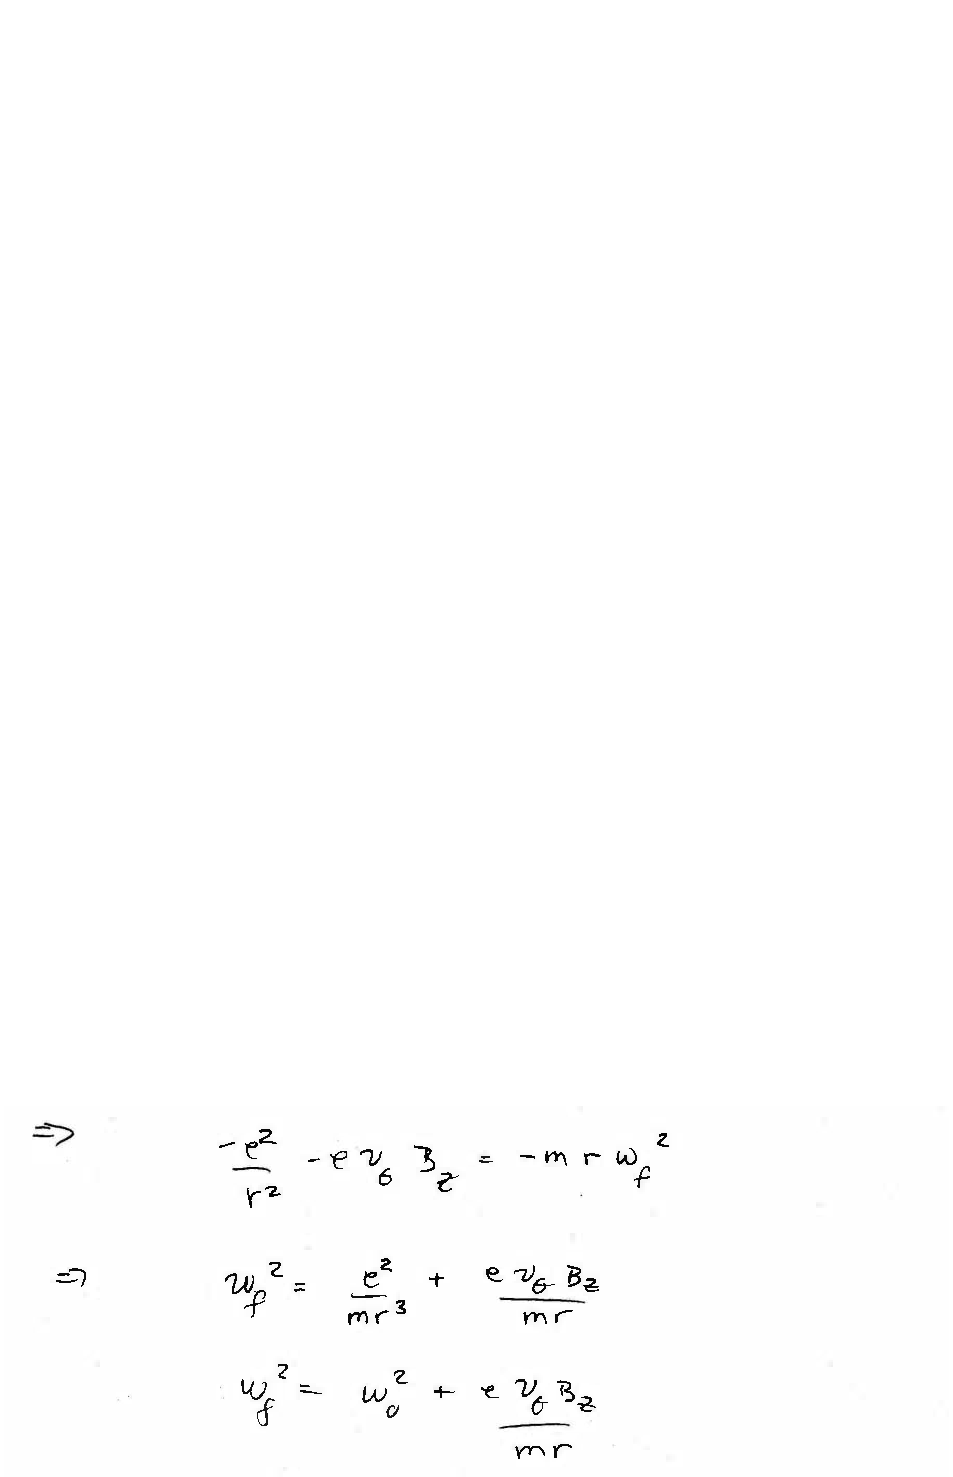
\includegraphics[width=\textwidth]{ps07_sol_02_4.pdf}\end{center}
\section{Problem \thesection: }
\subsection{Problem}
  A rod with a mass $m$ and a radius $R$ is mounted on two parallel rails of length a separated by a distance $\ell$, as shown in the figure below. The rod carries a current $I$ and rolls without slipping along the rails which are placed in a uniform magnetic field $\vec B$ directed into the page. If the rod is initially at rest, what is its speed as it leaves the rails?
  \begin{center}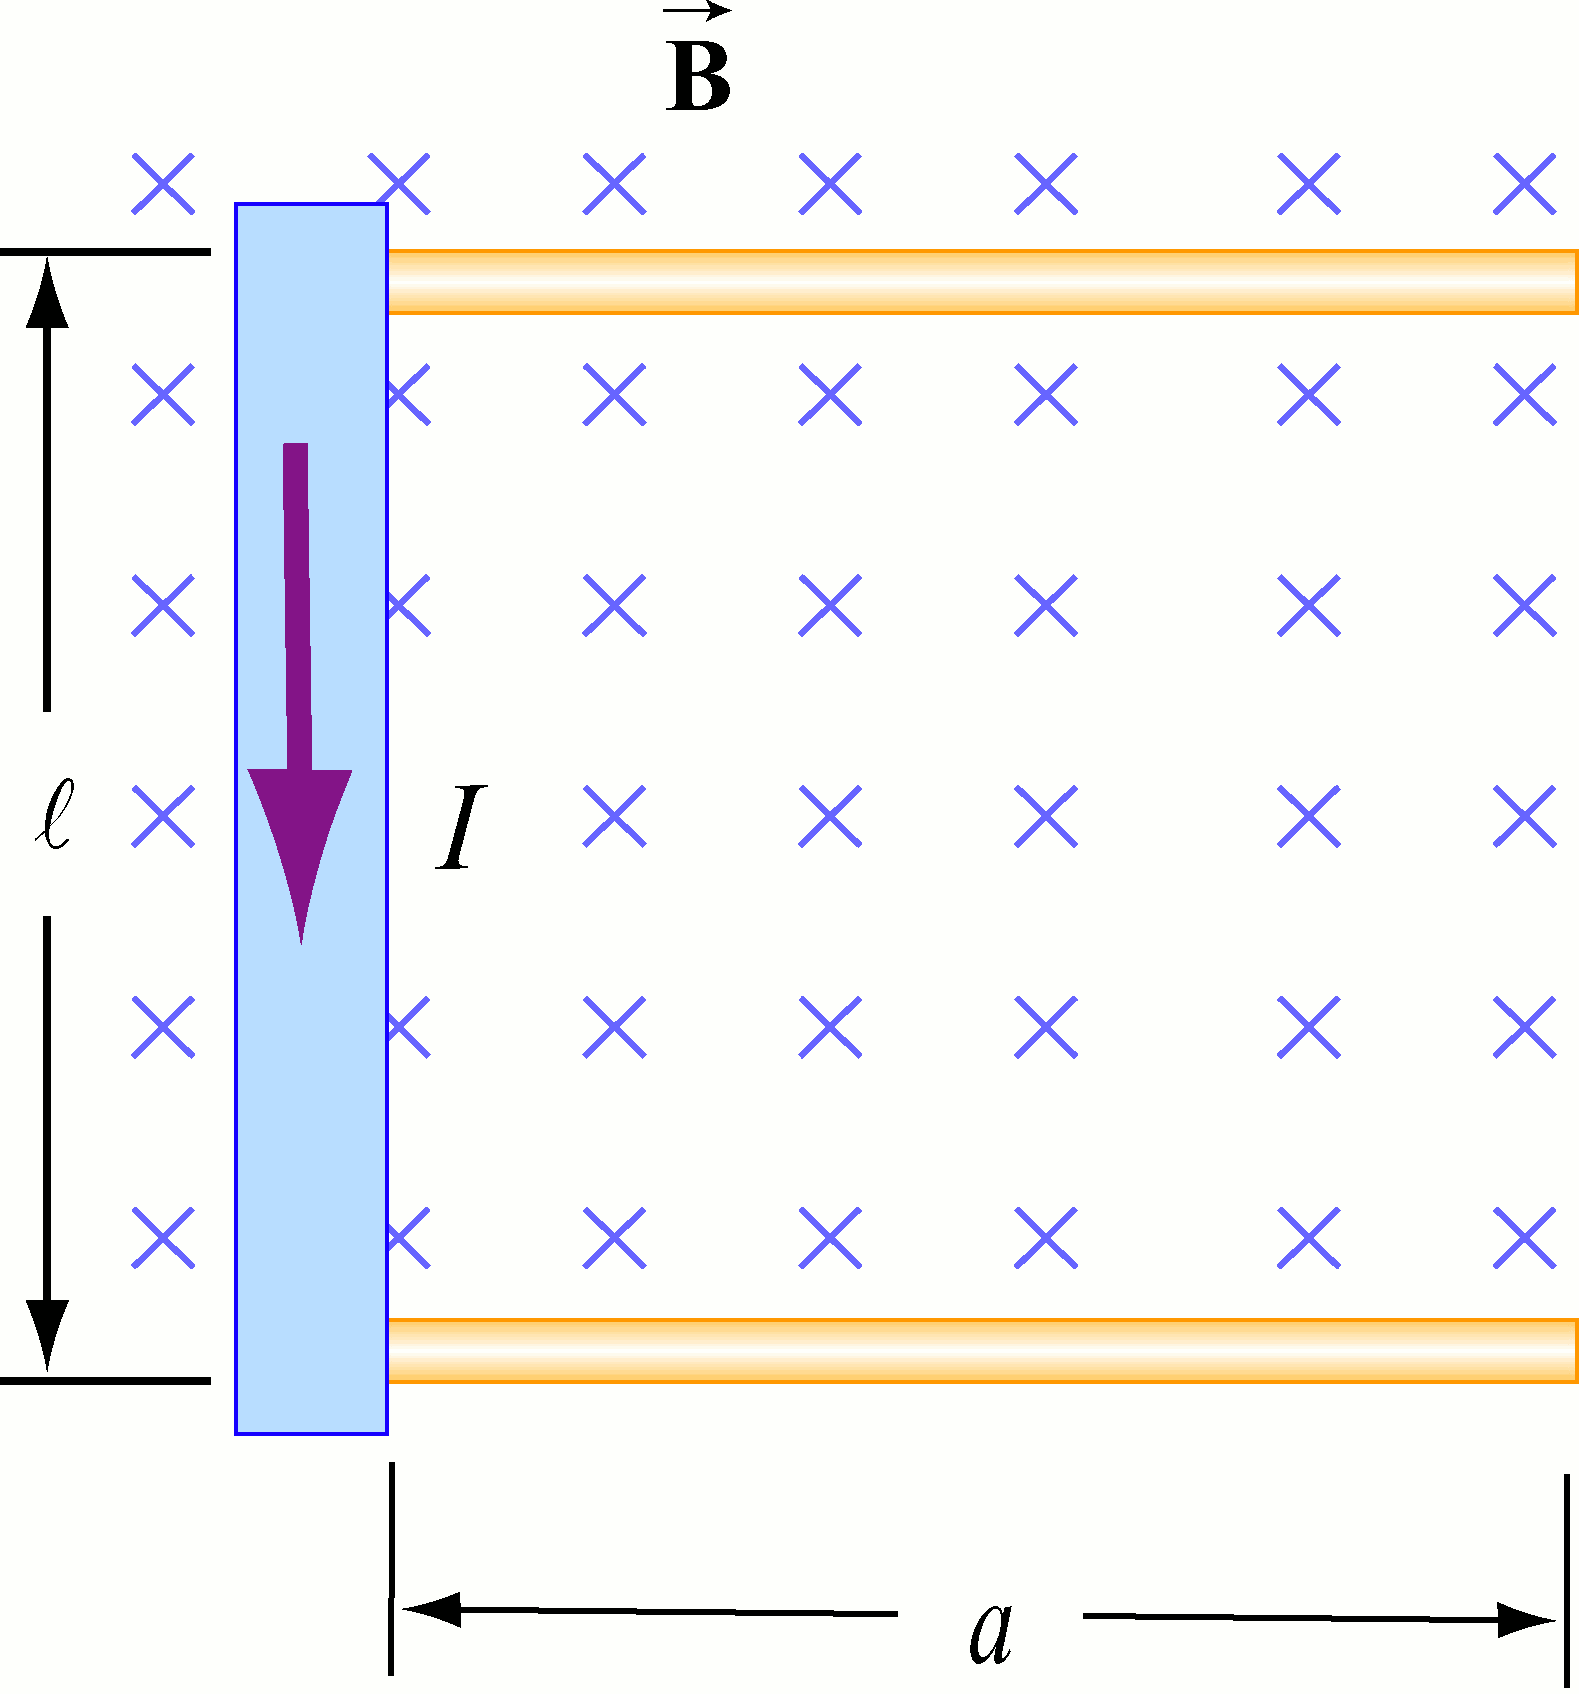
\includegraphics[width=0.33\textwidth]{ps07_03}\end{center}
\subsection{Solution}
  (In SI Units)

  \begin{wrapfigure}{r}{0.3\textwidth}
    \centering
    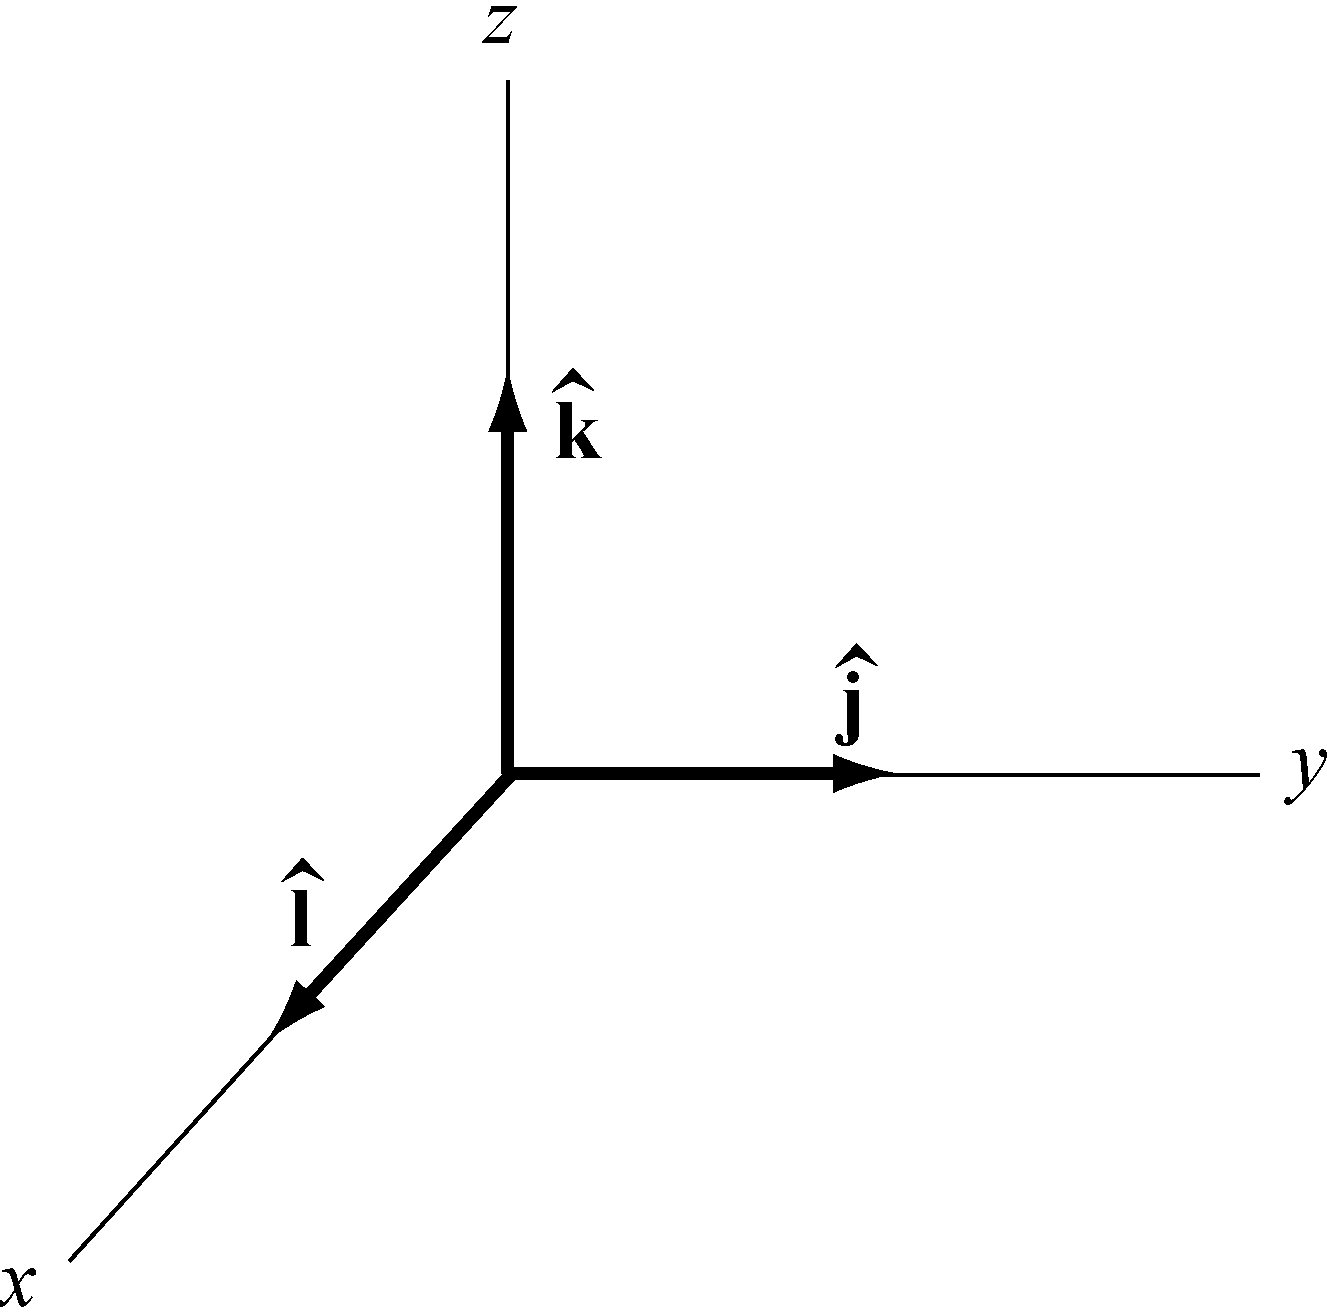
\includegraphics[width=0.28\textwidth]{ps07_sol_03_1}
  \end{wrapfigure}
  Using the coordinate system shown on the right, the magnetic force acting on the rod is given by
  $$\vec F_B = \vec{I \ell}\times \vec B = I (\ell \hat i) \times (-B\hat k) = I\ell B \hat j$$

  The total work done by the magnetic force on the rod as it moves through the region is
  $$W = \int \vec F_B\cdot d\vec s = F_B a = (I\ell B)a$$

  By the work-energy theorem, $W$ must be equal to the change in kinetic energy:
  $$\Delta K = \frac12 m v^2 + \frac12 I \omega^2$$
  where both translation and rolling are involved. Since the moment of inertia of the rod is given by $I = mR^2 / 2$, and the condition of rolling with slipping implies $\omega = v / R$, we have
  $$I \ell B a = \frac12 m v^2 + \frac12 \left(\frac{m R^2}{2}\right)\left(\frac{v}{R}\right)^2 = \frac12 m v^2 + \frac14 m v^2 = \frac34 m v^2$$

  Thus, the speed of the rod as it leaves the rails is
  $$v = \sqrt{\frac{4I\ell B a}{3m}}$$
\section{Problem \thesection: }
\subsection{Problem}
  A wire of arbitrary shape which is confined to the $x-y$ plane carries a current $I$ from point A to point B in the plane. Show that if a uniform magnetic field $B$ perpendicular to the $x-y$ plane is present, the force that the wire experiences is the same as that which would be felt by a wire running straight from A to B.
\subsection{Solution}
  \begin{center}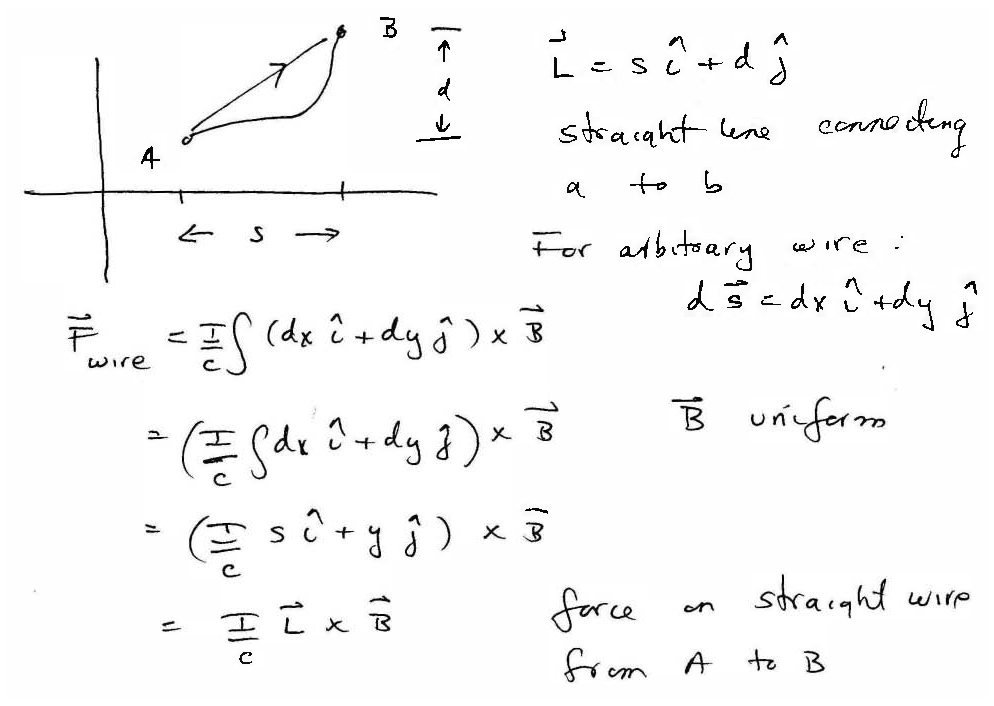
\includegraphics{ps07_sol_04_1.pdf}\end{center}
\section{Problem \thesection: }
\subsection{Problem}
  Calculate the divergence of the magnetic field of a straight wire in Cartesian coordinates.
\subsection{Solution}
  Put $r = \sqrt{x^2 + y^2}$.  With a little trigonometry, you should be able to convince yourself that
  \begin{align*}
    \hat\phi & = \hat y \cos\phi - \hat x\sin\phi \\
      & = \frac{x\hat y}{\sqrt{x^2 + y^2}} - \frac{y\hat x}{\sqrt{x^2 + y^2}},
  \end{align*}
  so
  $$\vec B = \frac{2I}{c}\left[\frac{x\hat y}{x^2 + y^2} - \frac{y\hat x}{x^2 + y^2}\right].$$
  The divergence of this field is
  \begin{align*}
    \vec\nabla \cdot \vec B & = \frac{2I}{c}\left[\frac{2yx}{(x^2 + y^2)^2} - \frac{2xy}{(x^2 + y^2)^2}\right] \\
      & = 0.
  \end{align*}
  We could have guessed this without doing any calculation: if we make any small box, there will be just as many field lines entering it as leaving.
\section{Problem \thesection: }
\subsection{Problem}
  Consider a cube which has identical resistors with resistance $R$ along each edge, as shown below.
  \begin{center}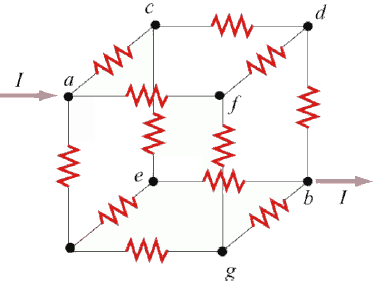
\includegraphics[width=0.33\textwidth]{ps07_06}\end{center}
  Find the equivalent resistance between points $a$ and $b$.
\subsection{Solution}
  From symmetry arguments, the current which enters $a$ must split evenly, with $I / 3$ going to each branch.  At the next junction, say $c$, $I / 3$ must further split evenly, with $I / 6$ going through the two paths $ce$ and $cd$.  The current going through the resistor in $db$ is the sum of the currents from $fd$ and $cd$: $I / 6 + I / 6 = I / 3$.

  Thus, the potential difference between $a$ and $b$ can be obtained as
  $$V_{ab} = V_{ac} + V_{cd} + V_{db} = \frac{I}{3}R + \frac{I}{6}R + \frac{I}{3}R = \frac56 IR$$
  hence the equivalent resistance is
  $$R_{\text{eq}} = \frac56 R.$$
\section{Problem \thesection: }
\subsection{Problem}
  \begin{center}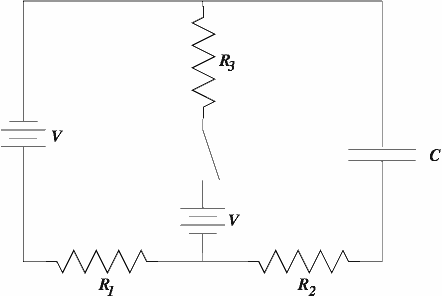
\includegraphics[width=0.5\textwidth]{ps07_07}\end{center}
  Suppose that the capacitor is initially charged.  The switch is closed at $t = 0$.  Find the current $I_{R_3}(t)$ through resistor $R_3$ (i.e., in the middle branch) as a function of time, and the charge in the capacitor $Q(t)$.  (Hint: this problem can be simplified greatly using Th\'evenin.  Compute $Q(t)$ first.)
\subsection{Solution}
  Version 1 takes $Q(0) = 0$.  Version 2 takes $Q(0) = CV$, which is more physically reasonable.
  \begin{center}
    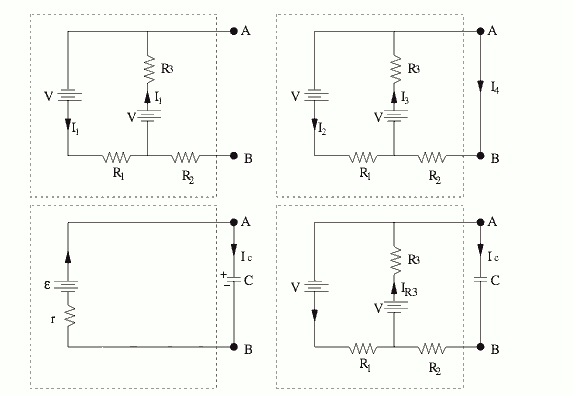
\includegraphics[width=0.8\textwidth]{ps07_sol_07_1} \\
    Figure 2: RC circuit network and it's Th\'evenin equivalence.
  \end{center}
  \begin{center}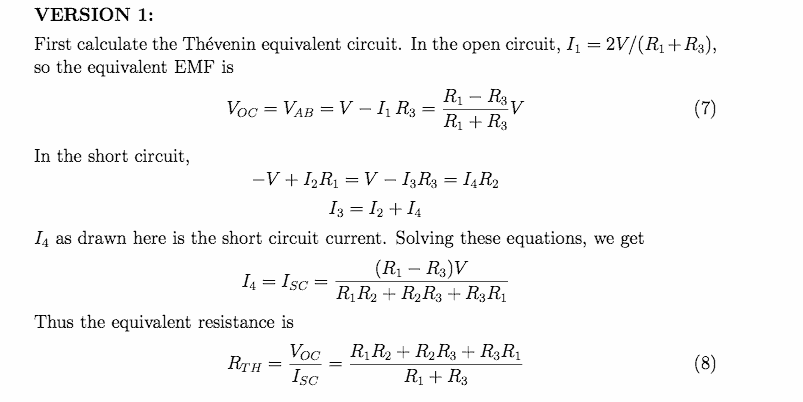
\includegraphics[width=\textwidth]{ps07_sol_07_2}\end{center}
  \begin{center}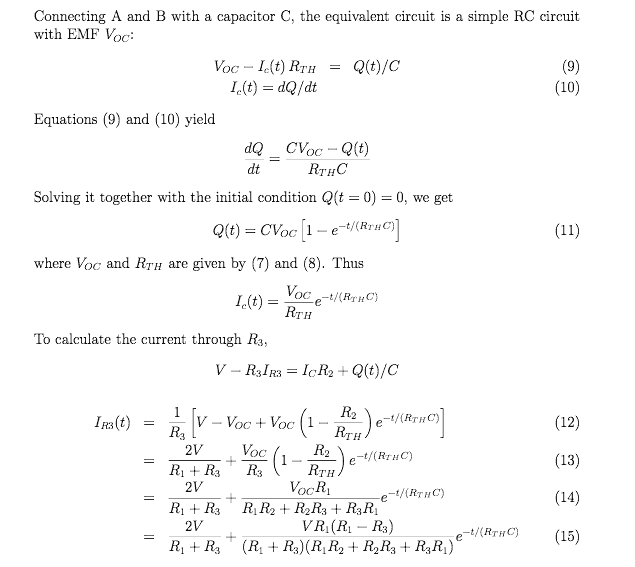
\includegraphics[width=\textwidth]{ps07_sol_07_3}\end{center}
  \begin{center}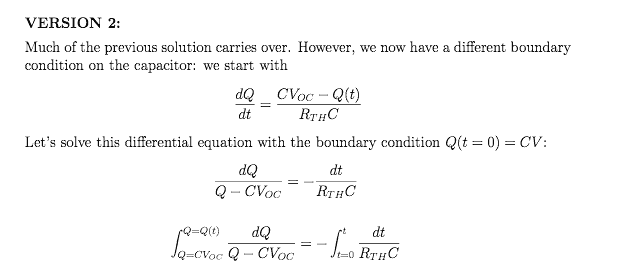
\includegraphics[width=\textwidth]{ps07_sol_07_4}\end{center}
  \begin{center}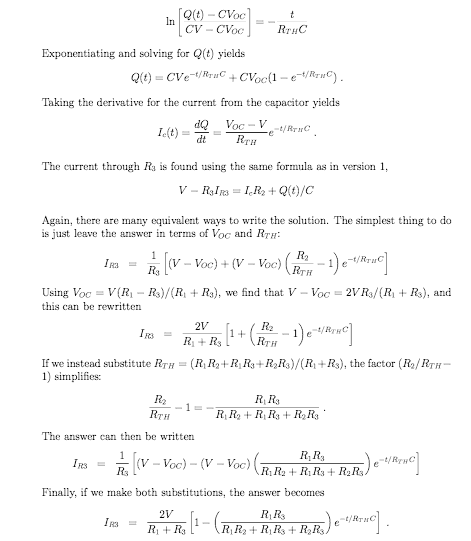
\includegraphics[width=\textwidth]{ps07_sol_07_5}\end{center}
\section{Problem \thesection: }
\subsection{Problem}
  Consider two parallel plates as shown in the sketch.  They each have a surface area $A$ and are separated by a distance $s$ that is small compared to the dimensions of the plate.  The top plate has a charge $+2Q$ deposited on it, while the bottom plate has charge $-Q$ deposited on it.  The two plates are not connected in any way.  For the purposes of this problem, assume that the charge densities are uniform on both surfaces of both plates, and ignore edge effects.
  \begin{center}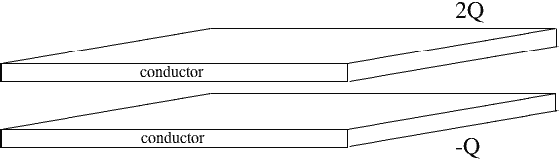
\includegraphics[width=0.75\textwidth]{ps07_08}\end{center}
  \begin{enumerate}[(a)]
    \item Find $\vec E$ between the two plates.
    \item Find the surface charge densities on the top and bottom faces of each of the two plates.
    \item Find $\vec E$ just above the top plate and just below the bottom plate.
    \item Show explicitly that the jump in $\vec E$ across each of the two plates is equal to $4\pi \sigma \hat n$ where $\sigma$ is the total surface charge density on that plate.
  \end{enumerate}
\subsection{Solution}
  \begin{center}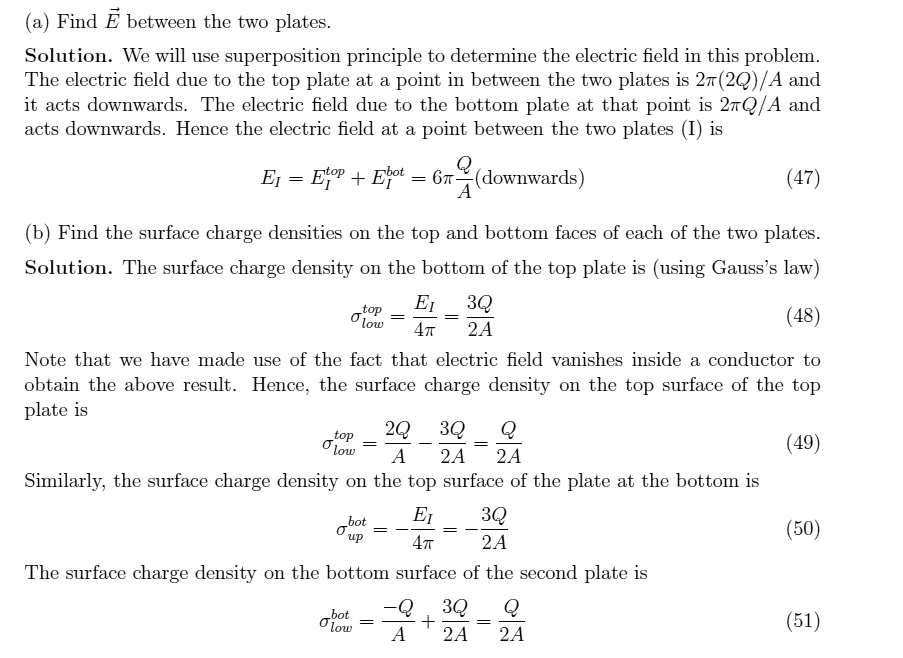
\includegraphics[width=\textwidth]{ps07_sol_08_1}\end{center}
  \begin{center}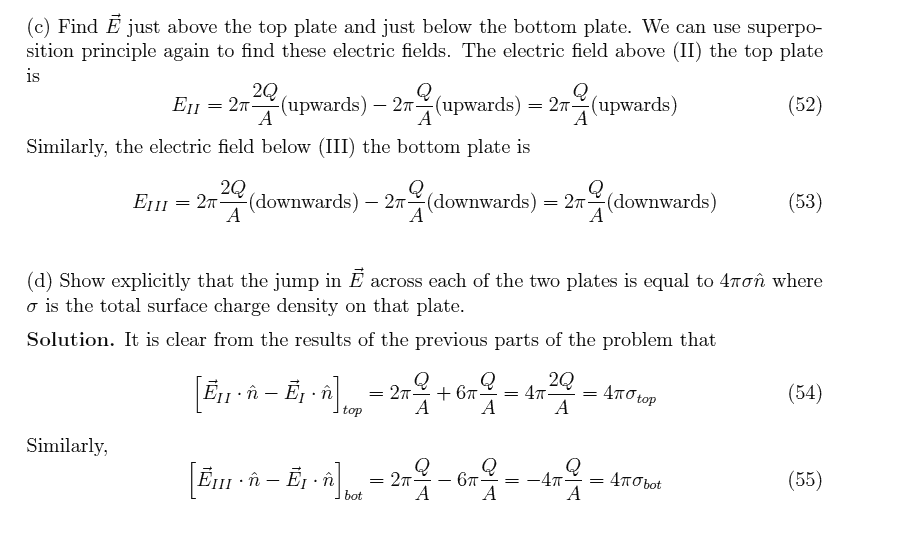
\includegraphics[width=\textwidth]{ps07_sol_08_2}\end{center}
\end{document}
